\section{Złożone kwadratury Newtona-Cotesa}
	\begin{frame}{Złożone kwadratury Newtona-Cotesa}
		Wzory N-C są niedogodne dla dużych $[a,\ b]-$ {\it piecewise technique}
        \begin{center}
      		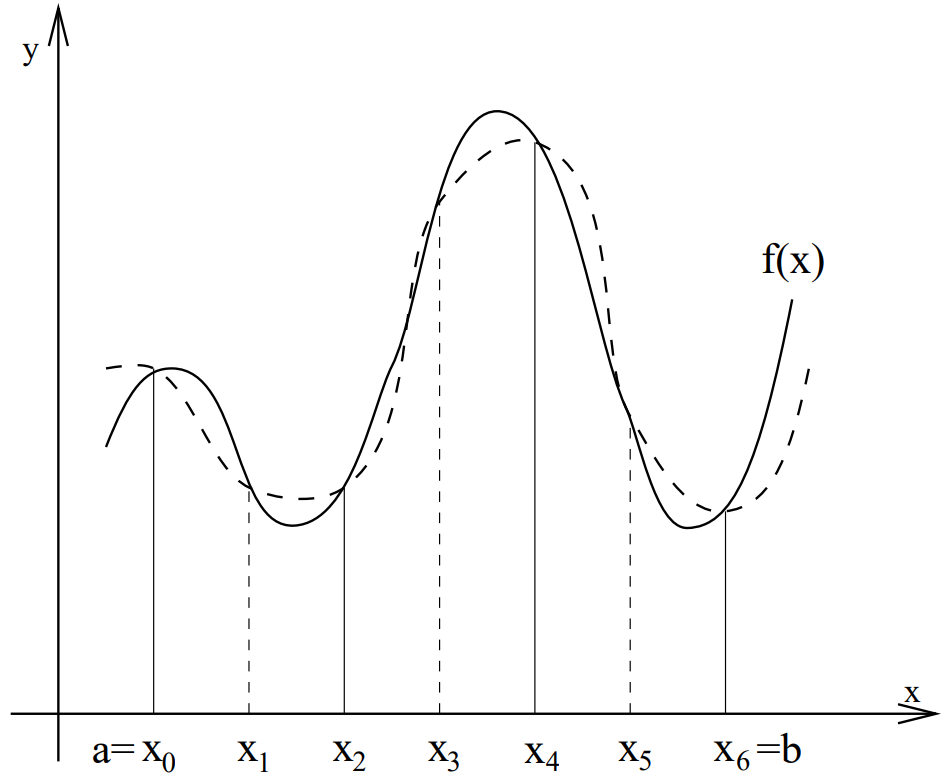
\includegraphics[width=0.6\linewidth]{img/6/image004.png}
      	\end{center}
	\end{frame}
%%%%%%%%%%%%%%%%%%%%%%%%%
	\begin{frame}
		Przedział $[a,\ b]$ podzielony na $n$ podprzedziałów $n=2m.$
        \newline
        (Simpson element. - 3 węzły)  
        $$
        h=\frac{b-a}{2m}, x_{i}=x_{0}+i\cdot h,\quad i=0, 1, 2, . . . , 2m
        $$
        \scalebox{0.85}{
          $\displaystyle
          \int_{a}^{b}f(x)dx=\sum_{j=1}^{m}\int_{x_{2j-2}}^{x_{2j}}f(x)dx=\sum_{j=1}^{m}\{\frac{h}{3}[f(x_{2j-2})+4f(x_{2j-1})+f(x_{2j})]-\frac{h^{5}}{90}f^{(4)}(\eta_{j})\}
          $
        }

        $\eta\in(x_{2j-2},\ x_{2j})$
        \newline
        \newline
        $f(x_{2j})$ występuje w składowych dla: $[x_{2j-2},\ x_{2j}]  [x_{2j},\ x_{2j+2}]$ i stąd:
        \newline

        \scalebox{0.9}{
          $\displaystyle
          \int_{a}^{b}f(x)dx=\frac{h}{3}[f(x_{0})+4\sum_{j=1}^{m}f(x_{2j-1})+\sum_{j=1}^{m-1}f(x_{2j})+f(x_{2m})]-\frac{h^{5}}{90}\sum_{j=1}^{m}f^{(4)}(\eta_{j})
          $
        }
	\end{frame}
%%%%%%%%%%%%%%%%%%%%%%%%%
	\begin{frame}{Błąd dla wzoru złożonego}
      \textbf{z tw. o wartości średniej: ( $f^{(4)}$ - ciągła )}
      $$
      \min_{x\in[a,b]}f^{(4)}(x)\leq f^{(4)}(\eta_{j})\leq \max_{x\in[a,b]}f^{(4)}(x) ,\quad \eta_{j}\in(x_{2j-2},\ x_{2j})
      $$
      \newline
	  dla każdego przedziału w wyniku dodawania:
      \begin{center}
        $\displaystyle
        m\cdot\min_{x\in[a,b]}f^{(4)}(x)\leq\sum_{j=1}^{m}f^{(4)}(\eta_{j})\leq m\cdot \max_{x\in[a,b]}f^{(4)}(x),
        $
        \newline
        $\displaystyle
        \min_{x\in[a,b]}f^{(4)}(x)\leq\frac{1}{m}\sum_{j=1}^{m}f^{(4)}(\eta_{j})\leq \max_{x\in[a,b]}f^{(4)}(x),
        $
      \end{center}
        
    \end{frame}
%%%%%%%%%%%%%%%%%%%%%%%%%
	\begin{frame}
      $$
      \textnormal{(z tw.) }\exists\mu\in(a,\ b) :\quad f^{(4)}(\mu)=\frac{1}{m}\sum_{j=1}^{m}f^{(4)}(n_{j}) \quad \Rightarrow
      $$

      $\displaystyle
      \qquad\quad E=-\frac{h^{5}}{90} \cdot m\cdot f^{(4)}(\mu) ,\quad m= \frac{b-a}{2h} \quad \Rightarrow
      $
      \begin{exampleblock}{}
      	\[
        	E=-\frac{h^{4}(b-a)}{180}f^{(4)}(\mu)
        \]
      \end{exampleblock}
%       \begin{center}
%       \fbox{$E=-\displaystyle $}
%       \end{center}
    \end{frame}
%%%%%%%%%%%%%%%%%%%%%%%%%
	\begin{frame}{Wpływ błędu wyznaczania $f(x)$}
        $$
        f(x_{i})=f^{\star}(x_{i})+e_{i};\quad i=0, 1, 2, . . ., 2m
        $$
        \newline
        (błąd zaokrąglenia $|\epsilon_{i}|<\epsilon$)
        \newline
		błąd wzoru złożonego:
        \scalebox{0.72}{
          $\displaystyle \Upsilon=|\frac{h}{3}[e_{0}+4\sum_{j=1}^{m}e_{2j-1}+2\sum_{j=1}^{m-1}e_{2j}+e_{2m}]|\leq\frac{h}{3}[\epsilon+4m\epsilon+2(m+1)\epsilon+\epsilon]=2mh\epsilon= \fbox{$(b-a)\cdot\epsilon$}$
		}
        
        \quad $\bullet$ nie zalezy od $h$
        
		\quad $\bullet$ $h\rightarrow 0$ to stabilna
        
		\quad $\bullet$ nie mylić z błędem metody!!!!
        
		\quad $\bullet$ stabilność metody ze względu na błędy zaokrągleń (reprezentacji) - cecha procedur calkowania numerycznego!\newline (nie ma jej np. różniczkowanie!)\newline

		\textbf{{\it Zadanie}: wzory złożone dla trapezów i prostokątów}
        
    \end{frame}
%%%%%%%%%%%%%%%%%%%%%%%%%